\documentclass[11pt, letterpaper]{article}
\pagestyle{empty}
\usepackage[a4paper, margin=1cm]{geometry} % Adjust margins as needed
\usepackage{multirow}
\usepackage{enumitem}
\usepackage{graphicx}
\usepackage{minted}
\usepackage[most]{tcolorbox}
\usepackage{etoolbox}
\usepackage[table]{xcolor}
\usepackage{tabularx}
\usepackage{microtype}
\usepackage{tikz}
\usepackage[md]{titlesec}
\setminted{fontsize=\large}
\usemintedstyle{bw}
\newcommand{\includeminted}[3]
{
  \begin{center}
  \textbf{#1}
  \vspace{-5pt}
  \inputminted[linenos, breaklines]{#2}{#3}
  \end{center}
}

\newcommand{\mintbox}[3]
{
  \begin{center}
  \textbf{#1}
  \vspace{-5pt}
  \begin{tcolorbox}
  \inputminted[]{#2}{#3}
  \end{tcolorbox}
  \end{center}
}

\title{Exam revision}
\author{}
\date{}

\begin{document}
\normalsize
\section{Lab 10}
\includeminted{Figure 1: Array.h}{cpp}{../10/src/Array.h}
\clearpage
\section{Lab 11}
\includeminted{Figure 2: DoublyLinkedList.h}{cpp}{../11/src/DoublyLinkedList.h}
\clearpage
\includeminted{Figure 3: DoublyLinkedListIterator.h}{cpp}{../11/src/DoublyLinkedListIterator.h}
\clearpage
\section{Lab 12}
\includeminted{Figure 4: BTree.h}{cpp}{../12/src/BTree.h}
\clearpage
\includeminted{Figure 5: TreeDecorator.h}{cpp}{../12/src/TreeDecorator.h}
\clearpage
\section*{Revision Questions}
\setlength{\parskip}{0.5em}

\newtcolorbox{answerspace}{
  colback=white,
  colframe=black,
  boxrule=0.5pt,
  left=2mm,
  right=2mm,
  top=1mm,
  bottom=1mm,
  enhanced,
  height=3cm,
  breakable
}

\begin{enumerate}[leftmargin=*, label=\textbf{\arabic*.}]
  \item What is the difference between a shallow copy and a deep copy?
    \begin{answerspace}
    \end{answerspace}

  \item Why should you use \texttt{make\_shared} and \texttt{make\_unique} when using smart pointers?
    \begin{answerspace}
    \end{answerspace}

  \item What is the point of \texttt{perfect forwarding}, and why should you use \texttt{std::forward} to forward arguments?
    \begin{answerspace}
    \end{answerspace}

  \item Give all the function signatures of a \texttt{Node} class, and where it could be used for a copy constructor, copy assignment operator, move constructor and move assignment operator.
    \begin{answerspace}
    \end{answerspace}

  \item Explain mutually dependent classes in C++ and give an example.
    \begin{answerspace}
    \end{answerspace}

  \item What are the dangers of using circular references with \texttt{shared\_ptr}?
    \begin{answerspace}
    \end{answerspace}
\clearpage
  \item How can we construct a tree where all nodes have the same degree?
    \begin{answerspace}
    \end{answerspace}

  \item What is the difference between l-value references and r-value references?
    \begin{answerspace}
    \end{answerspace}

  \item What is a key concept of abstract data types?
    \begin{answerspace}
    \end{answerspace}

  \item What must a value-based data type define in C++?
    \begin{answerspace}
    \end{answerspace}

  \item What is an object adapter?
    \begin{answerspace}
    \end{answerspace}

  \item What is the difference between copy constructor and assignment operator and how do we guarantee safe function?
    \begin{answerspace}
    \end{answerspace}

  \item What is the best-case, worst-case and average case lookup in a binary tree?
    \begin{answerspace}
    \end{answerspace}

  \item What are reference data members and how do we initialize them?
    \begin{answerspace}
    \end{answerspace}

  \item What is RAII and how is it leveraged in C++?
    \begin{answerspace}
    \end{answerspace}

\end{enumerate}
\clearpage
\section*{Tree Traversal Practice}

\noindent\textbf{Instructions:}  
For each tree below, write the \textbf{node number} inside each circle according to the specified traversal order.

\vspace{1em}

\begin{enumerate}[leftmargin=*]
  \item \textbf{Pre-order traversal:} Number the nodes in pre-order.
  \item \textbf{In-order traversal:} Number the nodes in in-order.
  \item \textbf{Post-order traversal:} Number the nodes in post-order.
\end{enumerate}

\vspace{2em}

\newcommand{\binarytree}{
\begin{center}
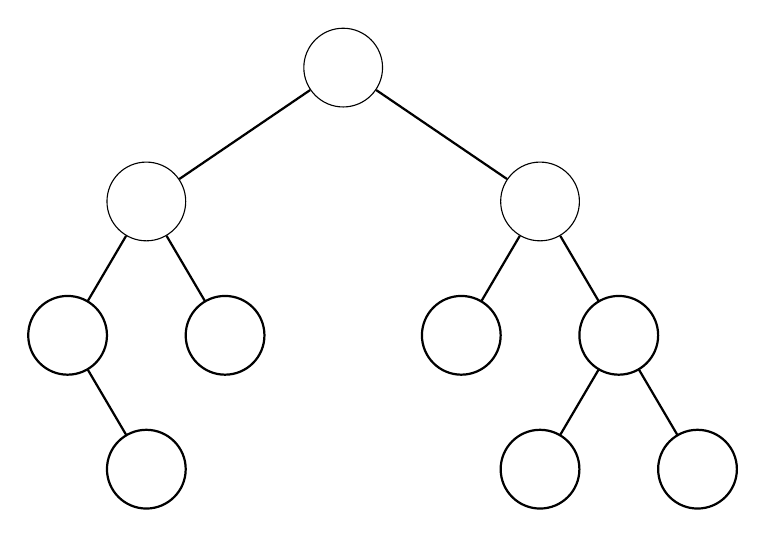
\begin{tikzpicture}[level distance=1.7cm,
  level 1/.style={sibling distance=5cm},
  level 2/.style={sibling distance=2cm},
  every node/.append style={circle,draw,minimum size=1cm, font=\large, fill=white, text=black},
  edge from parent/.style={draw,thick}]
\node {} % root
  child { node {} % left child of root
    child { % left subtree: left child
      node {} % left child
        child[missing] % no left child
        child { node {} } % right child only
    }
    child { node {} } % right child of left
  }
  child { node {} % right child of root
    child { node {} } % left
    child { % right subtree: right child
      node {}
        child { node {} }
        child { node {} }
    }
  };
\end{tikzpicture}
\end{center}
}

% Pre-order Tree
\subsection*{1. Pre-order Traversal}
\binarytree
\vspace{1.5cm}


% In-order Tree
\subsection*{2. In-order Traversal}
\binarytree
\vspace{1.5cm}

\clearpage

% Post-order Tree
\subsection*{3. Post-order Traversal}
\binarytree
\vspace{1.5cm}

\end{document}
